% Options for packages loaded elsewhere
\PassOptionsToPackage{unicode}{hyperref}
\PassOptionsToPackage{hyphens}{url}
\PassOptionsToPackage{dvipsnames,svgnames,x11names}{xcolor}
%
\documentclass[
  letterpaper,
  DIV=11,
  numbers=noendperiod]{scrartcl}

\usepackage{amsmath,amssymb}
\usepackage{iftex}
\ifPDFTeX
  \usepackage[T1]{fontenc}
  \usepackage[utf8]{inputenc}
  \usepackage{textcomp} % provide euro and other symbols
\else % if luatex or xetex
  \usepackage{unicode-math}
  \defaultfontfeatures{Scale=MatchLowercase}
  \defaultfontfeatures[\rmfamily]{Ligatures=TeX,Scale=1}
\fi
\usepackage{lmodern}
\ifPDFTeX\else  
    % xetex/luatex font selection
\fi
% Use upquote if available, for straight quotes in verbatim environments
\IfFileExists{upquote.sty}{\usepackage{upquote}}{}
\IfFileExists{microtype.sty}{% use microtype if available
  \usepackage[]{microtype}
  \UseMicrotypeSet[protrusion]{basicmath} % disable protrusion for tt fonts
}{}
\makeatletter
\@ifundefined{KOMAClassName}{% if non-KOMA class
  \IfFileExists{parskip.sty}{%
    \usepackage{parskip}
  }{% else
    \setlength{\parindent}{0pt}
    \setlength{\parskip}{6pt plus 2pt minus 1pt}}
}{% if KOMA class
  \KOMAoptions{parskip=half}}
\makeatother
\usepackage{xcolor}
\setlength{\emergencystretch}{3em} % prevent overfull lines
\setcounter{secnumdepth}{-\maxdimen} % remove section numbering
% Make \paragraph and \subparagraph free-standing
\ifx\paragraph\undefined\else
  \let\oldparagraph\paragraph
  \renewcommand{\paragraph}[1]{\oldparagraph{#1}\mbox{}}
\fi
\ifx\subparagraph\undefined\else
  \let\oldsubparagraph\subparagraph
  \renewcommand{\subparagraph}[1]{\oldsubparagraph{#1}\mbox{}}
\fi


\providecommand{\tightlist}{%
  \setlength{\itemsep}{0pt}\setlength{\parskip}{0pt}}\usepackage{longtable,booktabs,array}
\usepackage{calc} % for calculating minipage widths
% Correct order of tables after \paragraph or \subparagraph
\usepackage{etoolbox}
\makeatletter
\patchcmd\longtable{\par}{\if@noskipsec\mbox{}\fi\par}{}{}
\makeatother
% Allow footnotes in longtable head/foot
\IfFileExists{footnotehyper.sty}{\usepackage{footnotehyper}}{\usepackage{footnote}}
\makesavenoteenv{longtable}
\usepackage{graphicx}
\makeatletter
\def\maxwidth{\ifdim\Gin@nat@width>\linewidth\linewidth\else\Gin@nat@width\fi}
\def\maxheight{\ifdim\Gin@nat@height>\textheight\textheight\else\Gin@nat@height\fi}
\makeatother
% Scale images if necessary, so that they will not overflow the page
% margins by default, and it is still possible to overwrite the defaults
% using explicit options in \includegraphics[width, height, ...]{}
\setkeys{Gin}{width=\maxwidth,height=\maxheight,keepaspectratio}
% Set default figure placement to htbp
\makeatletter
\def\fps@figure{htbp}
\makeatother

\KOMAoption{captions}{tableheading}
\makeatletter
\@ifpackageloaded{caption}{}{\usepackage{caption}}
\AtBeginDocument{%
\ifdefined\contentsname
  \renewcommand*\contentsname{Table of contents}
\else
  \newcommand\contentsname{Table of contents}
\fi
\ifdefined\listfigurename
  \renewcommand*\listfigurename{List of Figures}
\else
  \newcommand\listfigurename{List of Figures}
\fi
\ifdefined\listtablename
  \renewcommand*\listtablename{List of Tables}
\else
  \newcommand\listtablename{List of Tables}
\fi
\ifdefined\figurename
  \renewcommand*\figurename{Figure}
\else
  \newcommand\figurename{Figure}
\fi
\ifdefined\tablename
  \renewcommand*\tablename{Table}
\else
  \newcommand\tablename{Table}
\fi
}
\@ifpackageloaded{float}{}{\usepackage{float}}
\floatstyle{ruled}
\@ifundefined{c@chapter}{\newfloat{codelisting}{h}{lop}}{\newfloat{codelisting}{h}{lop}[chapter]}
\floatname{codelisting}{Listing}
\newcommand*\listoflistings{\listof{codelisting}{List of Listings}}
\makeatother
\makeatletter
\makeatother
\makeatletter
\@ifpackageloaded{caption}{}{\usepackage{caption}}
\@ifpackageloaded{subcaption}{}{\usepackage{subcaption}}
\makeatother
\ifLuaTeX
  \usepackage{selnolig}  % disable illegal ligatures
\fi
\usepackage{bookmark}

\IfFileExists{xurl.sty}{\usepackage{xurl}}{} % add URL line breaks if available
\urlstyle{same} % disable monospaced font for URLs
\hypersetup{
  pdftitle={London SDE/AIC Programme: Introduction and Proposed Use-Cases},
  colorlinks=true,
  linkcolor={blue},
  filecolor={Maroon},
  citecolor={Blue},
  urlcolor={Blue},
  pdfcreator={LaTeX via pandoc}}

\title{London SDE/AIC Programme\texttt{:} Introduction and Proposed
Use-Cases}
\author{Dr.~Joe Zhang \and Prof.~James Teo \and Dr.~Jorge
Cardoso \and Jawad Chaudhry \and Sigal Hachlili}
\date{}

\begin{document}
\maketitle

\emph{Version 0.5 (last updated 2024 Apr 7)}

\subsection{Introduction}\label{introduction}

The \href{https://www.aicentre.co.uk/}{London AI Centre} (AIC) has been
commissioned to join the London Secure Data Environment (SDE) programme
for its latest phase: to build on existing infrastructural work, and
extend AI technologies and advanced analytics capabilities to
stakeholders and environments across London. This \emph{living document}
summarises the latest state of planning for the programme, as a
transparent aid to internal stakeholders, and collaborators in
Integrated Care Boards and the wider London NHS ecosystem.

\subsection{What is the London SDE?}\label{what-is-the-london-sde}

The London Secure Data Environment (SDE) programme is part of a national
effort to enable secure and more powerful analytics for NHS, academic,
and commercial users. Uniquely amongst regional peers, the London SDE
does not focus on a single research platform. Rather, it places a focus
on developing pan-London data infrastructure and capabilities that can
deliver value to patients, care providers, and commissioners. This is in
addition to building data environments that support commercial research
and development partnerships.

The SDE is presently led by \textbf{OneLondon}, as part of an
overarching London Health Data Strategy, coalescing around three
components (Figure~\ref{fig-sde-summary}).

\begin{enumerate}
\def\labelenumi{(\arabic{enumi})}
\item
  \textbf{London Data Service (LDS)}: hosted in North-East London, the
  LDS serves as a data engineering and service layer for pan-London
  primary care and secondary care data. It handles data extraction and
  linkage, and provisions data warehouses and secure analytics
  environments for both research and NHS users.
\item
  \textbf{DiscoverNOW Research/Analytics Environment}: run by Imperial
  College Healthcare Partners, DiscoverNOW supports governance and
  operation of secure research environments for academic, commercial,
  and NHS research and analytics.
\item
  \textbf{London AI Centre (AIC)}: a national centre of excellence for
  applied data science and AI, the AIC provides frontier technology for
  data enrichment, federated analytics, and deployment of machine
  learning tools, as well as expertise in health data and advanced
  analytics.
\end{enumerate}

\begin{figure}

\centering{

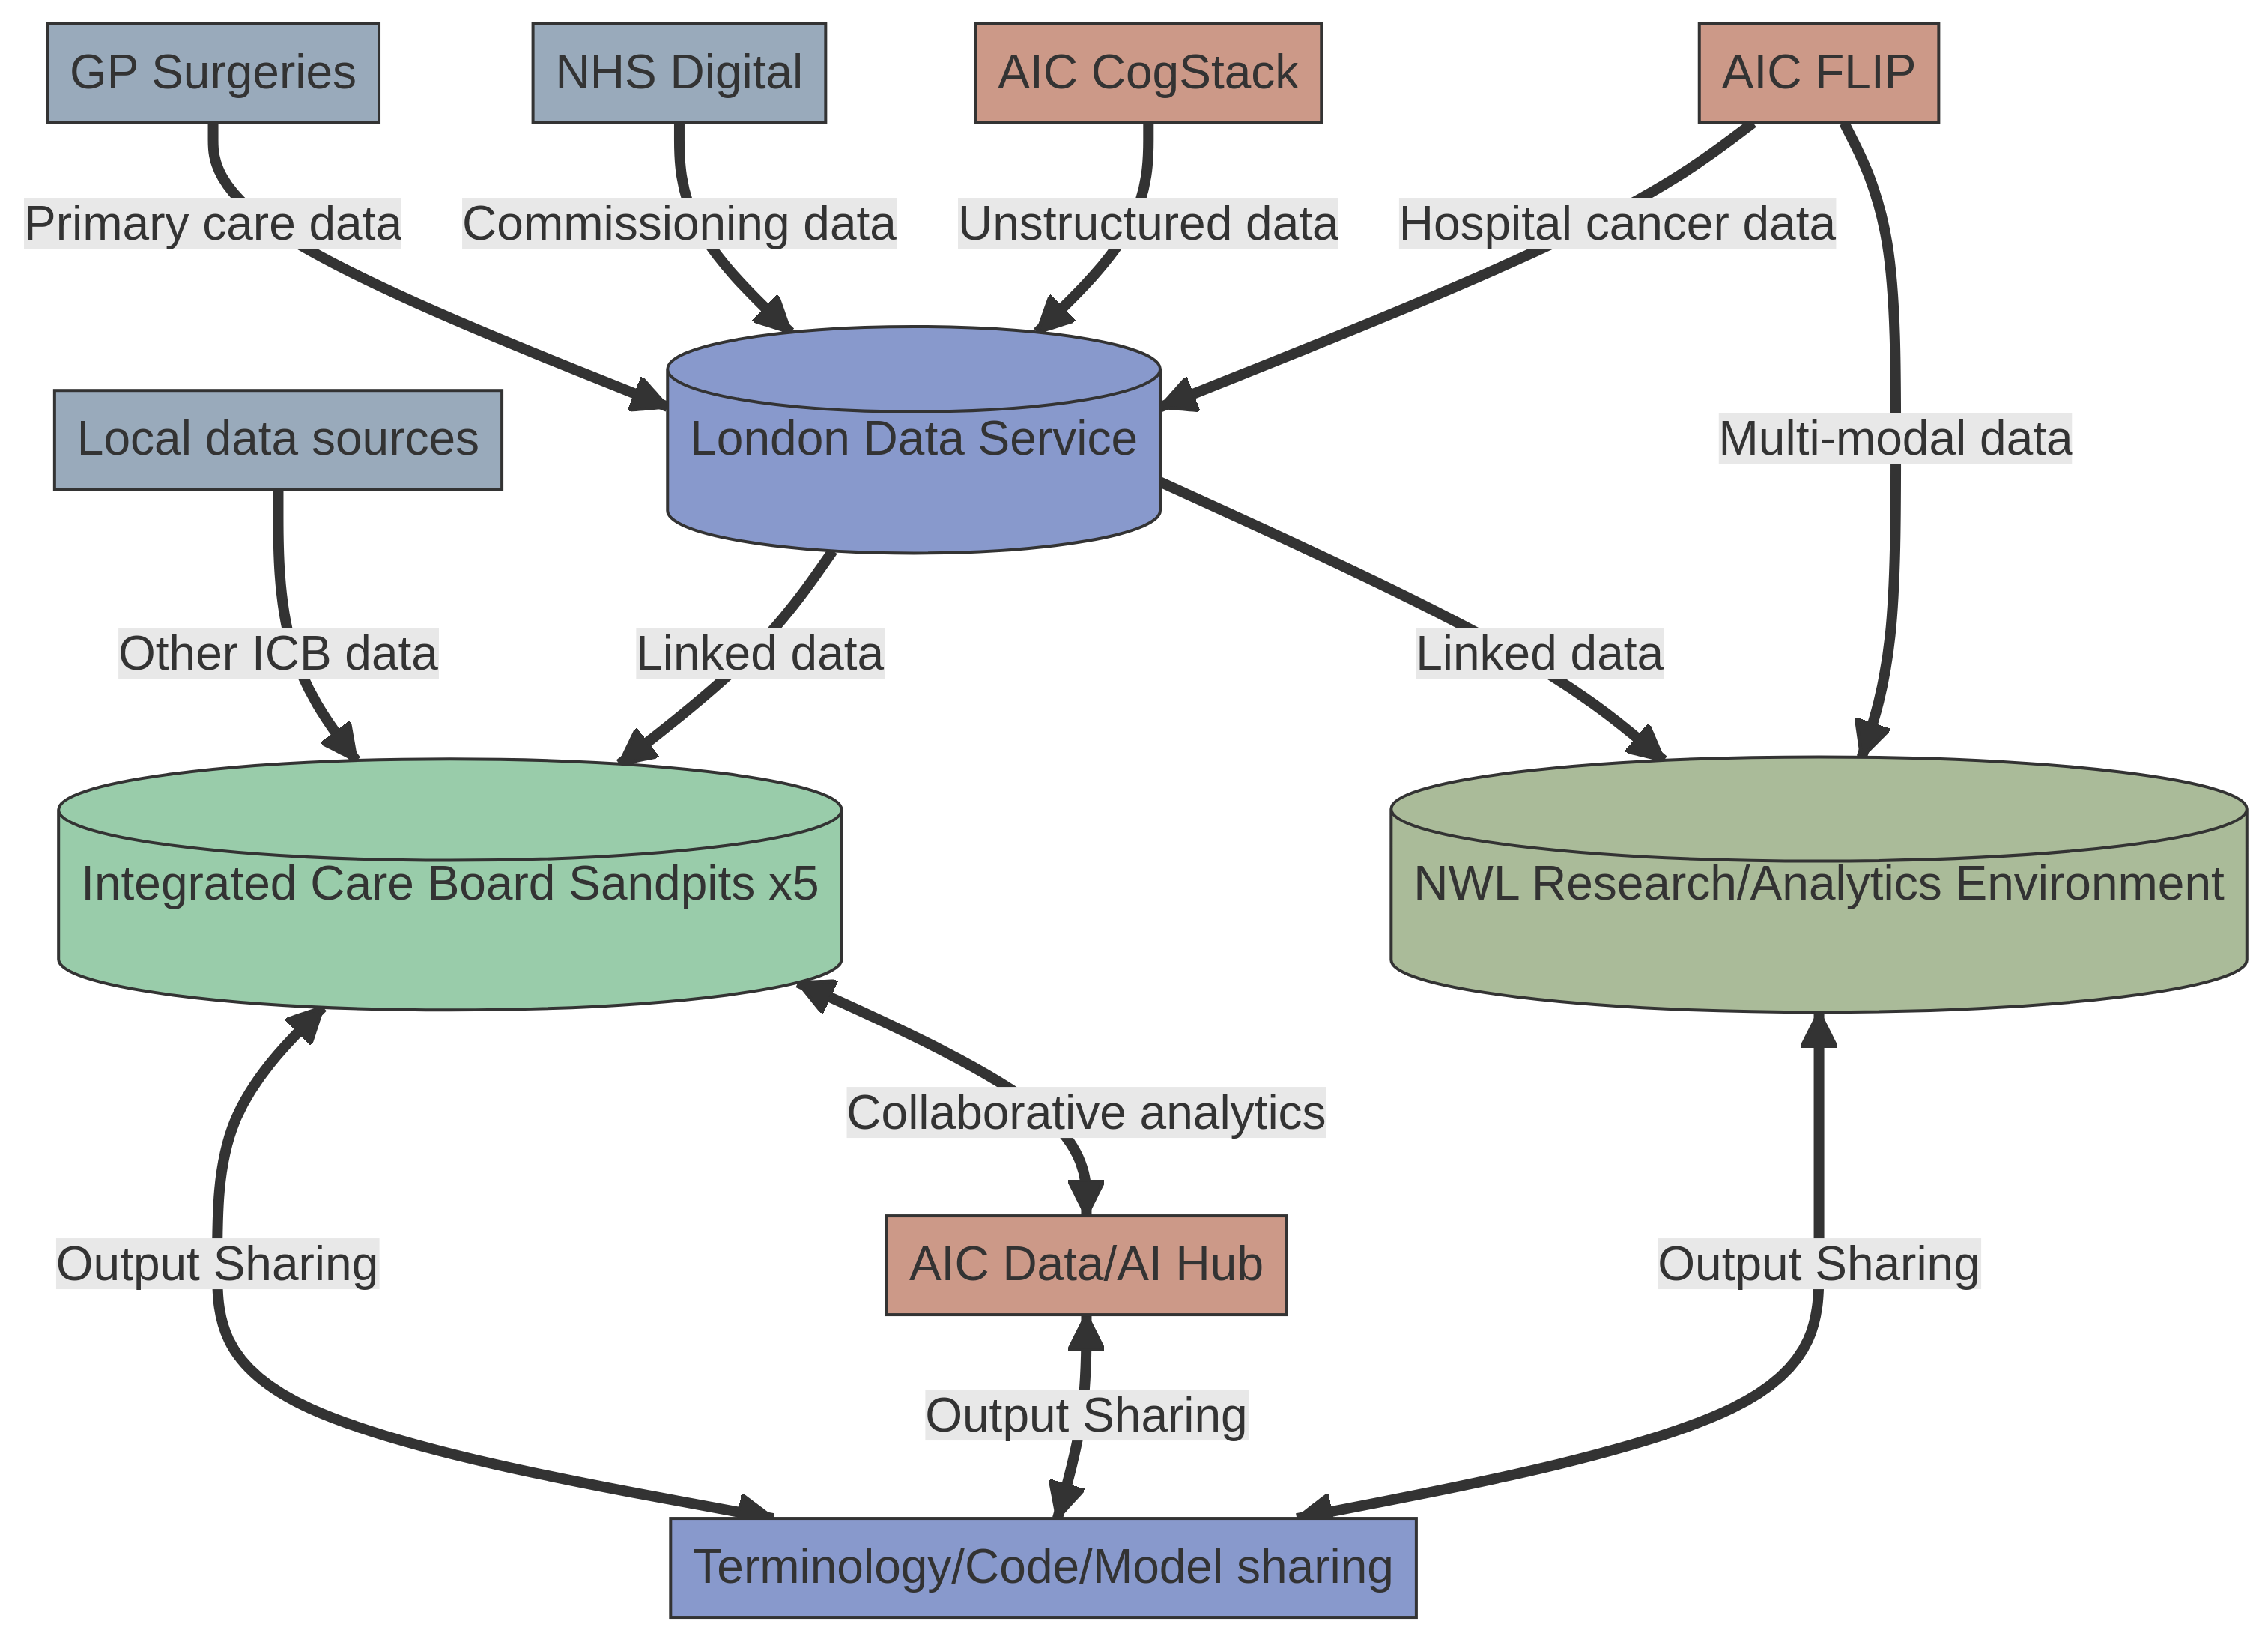
\includegraphics[width=7.9in,height=5.71in]{index_files/figure-latex/mermaid-figure-2.png}

}

\caption{\label{fig-sde-summary}Summary of SDE components and data
flows. Each London ICB is provisioned with its own data/analytics
environment through the LDS. FLIP = Federated Learning and
Interoperability Platform.}

\end{figure}%

\textsubscript{Source:
\href{https://d3london.github.io/sde_aic_docs/index.qmd.html}{Article
Notebook}}

\subsection{Technology and objectives}\label{technology-and-objectives}

\subsection{Proposed use-cases}\label{proposed-use-cases}



\end{document}
